\chapter{時間発展、保存則、結合スピン}

量子状態はヒルベルト空間内の固定点ではない。時間が経過するにつれてそれは動くが、規格化、確率、あるいは内積に符号化された識別可能性を失うことなく動かなければならない。これらの要請は量子力学の形式をほぼ決定づける。線形性は時間発展演算子を与え、確率保存はその演算子をユニタリにし、無限小ユニタリ変換はエルミート演算子によって生成される。その演算子がハミルトニアンである。我々はこれらの命題からSchr\"odinger方程式を導出し、エネルギー固有状態がどのように位相を蓄積するかを見て、その後この形式を二つの具体的な計算に適用する。すなわち、磁場中での一つのスピンの歳差運動と、結合したスピン対の二つの状態間の振動である。

\section{ヒルベルト空間内の線形運動}

時刻\(t\)における状態を\(\ket{\psi(t)}\)とする。時刻ゼロの状態との関係は線形であると仮定する：
\begin{equation}
\ket{\psi(t)}=U(t)\ket{\psi(0)}.
\end{equation}
この線形性は公理であり、より基本的な何かから導かれる定理ではない。これは量子力学の実験的に成功した部分であり、これを置き換えようとする試みは一般に確率か保存則のいずれかを危険にさらす。選んだ基底において、\(U(t)\)は単に時間依存する行列である。

双対ベクトルは共役規則に従う。もし
\begin{equation}
\ket{\phi(t)}=U(t)\ket{\phi(0)},
\end{equation}
ならば
\begin{equation}
\bra{\phi(t)}=\bra{\phi(0)}U^\dagger(t).
\end{equation}
である。行列に対して、ダガーは複素共役の後に転置を意味する。したがってブラは、双対空間で表されたケットと同じ発展則を担う。

\subsection{確率保存はユニタリ性を意味する}

規格化された状態は全確率1を表す：
\begin{equation}
\braket{\psi(t)}{\psi(t)}=1.
\end{equation}
時間発展はこのノルムを保存しなければならない。実際、すべてのベクトルのノルムを保存する線形写像はすべての内積も保存する。幾何学的には、二つのベクトルとその差の長さを保存することは、それらが作る三角形、したがってそれらの角度を保存する。複素ベクトル空間では、\(i\)の因子を持つ組み合わせも考慮することで同じ結論が導かれる。

したがって、任意の\(\ket{\phi}\)と\(\ket{\psi}\)に対して、
\begin{equation}
\braket{\phi(t)}{\psi(t)}
=
\braket{\phi(0)}{\psi(0)}.
\end{equation}
発展則を代入すると
\begin{equation}
\bra{\phi(0)}U^\dagger(t)U(t)\ket{\psi(0)}
=
\braket{\phi(0)}{\psi(0)}.
\end{equation}
この方程式がすべてのベクトル対に対して成り立つので、
\begin{equation}
\boxed{U^\dagger(t)U(t)=I}.
\end{equation}
このような演算子はユニタリである。スカラー版の類似物は大きさ1の複素数であり、
\begin{equation}
e^{i\theta}\bigl(e^{i\theta}\bigr)^*=1.
\end{equation}
ユニタリ演算子は純粋な位相の行列一般化である。それは状態をヒルベルト空間内で回転させることはできるが、引き伸ばしたり縮めたりすることはできない。

\section{無限小生成子}

有限の発展は非常に小さな時間刻みから構成される。経過時間を\(\epsilon\)とし、\(\epsilon^2\)のオーダーの項を無視できるほど小さいとする。経過時間ゼロでは何も起こらないので、
\begin{equation}
U(0)=I.
\end{equation}
主要な補正は\(\epsilon\)に比例しなければならない。これを慣習的な形で書くと
\begin{equation}
\boxed{U(\epsilon)=I-\frac{i\epsilon}{\hbar}H}.
\end{equation}
この段階で強制されるのは\(\epsilon\)の因子だけである。\(i\)、\(\hbar\)、および\(H\)という名称は、最終的に残る対象が標準的な規格化を持ちエルミートであるように選ばれている。

\begin{classroomqa}
\lecturetimestamp{00:12:46}
\audiencequestion{なぜプランク定数は身近な単位ではこれほど驚くほど小さな数なのですか？}
\lecturerresponse{その数値的な大きさは人間が選んだ単位を反映している。化学者は手に収まる容器に合う巨視的な量を選んだが、原子は人間よりはるかに小さい。それらの巨視的スケールに適合した単位では、作用の原子的量子は微小に見えなければならない。これは別個の力学的神秘ではなく、主に単位に組み込まれた歴史的・人間的スケールである。}
\end{classroomqa}

エルミート共役を取ると、
\begin{equation}
U^\dagger(\epsilon)
=I+\frac{i\epsilon}{\hbar}H^\dagger.
\end{equation}
ここで掛け合わせ、一次の項のみを保持する：
\begin{align}
U^\dagger(\epsilon)U(\epsilon)
&=
\left(I+\frac{i\epsilon}{\hbar}H^\dagger\right)
\left(I-\frac{i\epsilon}{\hbar}H\right) \\
&=
I+\frac{i\epsilon}{\hbar}\left(H^\dagger-H\right)
+O(\epsilon^2).
\end{align}
ユニタリ性はこの積が\(I\)に等しいことを要求するので、
\begin{equation}
\boxed{H^\dagger=H}.
\end{equation}
時間発展の無限小生成子はエルミートである。エルミート演算子は観測量を表すので、すべての力学系はその時間的運動を生成する観測量を持つ。これがハミルトニアンである。演算子には\(H\)を用い、その可能な測定値である固有値には\(E\)をとっておく。

\begin{classroomqa}
\lecturetimestamp{00:18:34}
\audiencequestion{なぜこの生成子をエネルギーと呼ぶべきなのですか？エネルギーとは\(p^2/2m\)、あるいは仕事をする能力ではないのですか？}
\lecturerresponse{それらは特別な古典的設定では有用な記述であるが、一般的な定義ではない。\(p^2/2m\)という表式は非相対論的自由粒子の運動エネルギーのみであり、電磁場に蓄えられたエネルギーなどのものを定義しない。抽象的な系に対して、エネルギーに要求すべき最初の普遍的特徴は保存である。我々はまもなく\(H\)の期待値が保存されることを証明し、その固有状態の位相も\(E=\hbar\omega\)を満たすであろう。これらの二つの事実が生成子をエネルギーと同定する。}
\end{classroomqa}

\section{小さな一歩からSchr\"odinger方程式へ}

無限小の更新は、すでに微分方程式の姿をしている。任意の時間の原点において、
\begin{equation}
\frac{d}{dt}\ket{\psi(t)}
=
\lim_{\epsilon\to0}
\frac{\ket{\psi(t+\epsilon)}-\ket{\psi(t)}}{\epsilon}.
\end{equation}
黒板ではまず\(t=0\)でこれを書き、原点をずらすと上記の一般形が得られる。

\begin{figure}[htbp]
\centering
\includegraphics[width=0.72\textwidth]{lecture_09_figure_03.png}
\caption{無限小の時間発展を微分方程式に変える差分商。}
\lectureframe{00:22:15}
\end{figure}

次を用いる。
\begin{equation}
\ket{\psi(t+\epsilon)}
=
\left(I-\frac{i\epsilon}{\hbar}H\right)\ket{\psi(t)}.
\end{equation}
すると
\begin{align}
\frac{d}{dt}\ket{\psi(t)}
&=
\lim_{\epsilon\to0}
\frac{\left(I-\frac{i\epsilon}{\hbar}H\right)\ket{\psi(t)}
-\ket{\psi(t)}}{\epsilon} \\
&=
-\frac{i}{\hbar}H\ket{\psi(t)}.
\end{align}
等価に、
\begin{equation}
\boxed{
i\hbar\frac{d}{dt}\ket{\psi(t)}
=H\ket{\psi(t)}
}.
\end{equation}
これがSchr\"odinger方程式である。\(H\)とある瞬間の状態がわかれば、それ以降の時刻の状態が決まる。後の測定に対する確率は、通常の測定規則から従う。

\section{エネルギー固有状態と回転する位相}

最も単純な解は、ハミルトニアンの固有ベクトルから始まる。
\begin{equation}
H\ket{\psi_E}=E\ket{\psi_E}.
\end{equation}

\begin{figure}[htbp]
\centering
\includegraphics[width=0.70\textwidth]{lecture_09_figure_04.png}
\caption{黒板上のエネルギー固有値方程式。}
\lectureframe{00:28:22}
\end{figure}

\(H\)は\(\ket{\psi_E}\)を同じ一次元の方向へ戻すので、時間発展はそれを別の固有ベクトルと混ぜることはできない。それはスカラーを掛けることしかできない。
\begin{equation}
\ket{\psi_E(t)}=f(t)\ket{\psi_E}.
\end{equation}
Schr\"odinger方程式に代入すると
\begin{align}
i\hbar\,\dot f(t)\ket{\psi_E}
&=
f(t)H\ket{\psi_E} \\
&=
E f(t)\ket{\psi_E}.
\end{align}
したがって
\begin{equation}
\dot f(t)=-\frac{iE}{\hbar}f(t),
\qquad
f(t)=e^{-iEt/\hbar},
\end{equation}
であり、
\begin{equation}
\boxed{
\ket{\psi_E(t)}
=e^{-iEt/\hbar}\ket{\psi_E(0)}
}.
\end{equation}
エネルギー固有状態は、ヒルベルト空間におけるそのレイが動かないという意味で定常である。しかしそのケットは位相を蓄積する。

指数関数は次のように書ける。
\begin{equation}
e^{-iEt/\hbar}
=
\cos\!\left(\frac{Et}{\hbar}\right)
-i\sin\!\left(\frac{Et}{\hbar}\right).
\end{equation}
負号と、正弦の中に余分な\(i\)が入らないことは、黒板上の計算の途中で修正された。角振動数は
\begin{equation}
\omega=\frac{E}{\hbar},
\qquad
\boxed{E=\hbar\omega}.
\end{equation}
等価に、通常の振動数\(\nu=\omega/(2\pi)\)を用いると、\(E=h\nu\)が成り立つ。

\begin{figure}[htbp]
\centering
\includegraphics[width=0.78\textwidth]{lecture_09_figure_05.png}
\caption{位相の解とエネルギー--振動数の関係が隣り合う黒板で展開される。}
\lectureframe{00:36:19}
\end{figure}

\begin{classroomqa}
\lecturetimestamp{00:34:43}
\audiencequestion{なぜ計算が必要とする前に、無限小演算子に\(i\)と\(\hbar\)の因子が挿入されたのか。}
\lecturerresponse{それらは答えを見越して選ばれた慣習である。\(i\)がなければ、ユニタリ性により生成子は反エルミートになる。\(i\)を掛けることで、それが実固有値をもつエルミートな観測量になる。因子\(\hbar\)はそれらの固有値にエネルギーの単位と規格化の慣習を与える。物理的な主張はユニタリ性であり、これらの因子はその生成子を標準形に置くものである。}
\end{classroomqa}

\begin{classroomqa}
\lecturetimestamp{00:36:18}
\audiencequestion{\(E=\hbar\omega\)は電磁波と光子だけに属するのか。}
\lecturerresponse{いいえ。光子は一つの重要な場合であるが、この関係はより一般的である。任意のハミルトニアン固有状態は角振動数\(E/\hbar\)の位相を獲得する。電磁場モードの振動数をその光子の振動数に結びつけるにはさらなる物理が必要だが、エネルギー--位相の関係自体はすでに量子の時間発展から従う。}
\end{classroomqa}

\section{エネルギー基底における重ね合わせ}

単一のエネルギー固有状態は全体位相だけによって変化し、全体位相は確率に影響を与え得ない。状態が複数のエネルギー固有ベクトルを含むときに興味深いダイナミクスが始まる。エルミートなハミルトニアンは完全な正規直交固有基底をもつので、
\begin{equation}
H\ket{\psi_n}=E_n\ket{\psi_n},
\qquad
\ket{\psi(0)}=\sum_n\alpha_n\ket{\psi_n}.
\end{equation}

\begin{figure}[htbp]
\centering
\includegraphics[width=0.72\textwidth]{lecture_09_figure_06.png}
\caption{任意の状態のハミルトニアン固有ベクトルによる展開。}
\lectureframe{00:38:35}
\end{figure}

線形性により、各成分は別々に発展できる。
\begin{equation}
\boxed{
\ket{\psi(t)}
=
\sum_n\alpha_n e^{-iE_n t/\hbar}\ket{\psi_n}
}.
\end{equation}
高エネルギーの成分は複素平面上を速く回り、低エネルギーの成分はよりゆっくり回る。測定可能な確率を変えるのは、状態全体に共通の位相ではなく、異なる\(E_n\)をもつ成分間の相対位相の変化である。

エネルギー基底では、
\begin{equation}
\begin{aligned}
H&=
\begin{pmatrix}
E_1&0&\cdots\\
0&E_2&\cdots\\
\vdots&\vdots&\ddots
\end{pmatrix},\\[0.6em]
U(t)&=
\begin{pmatrix}
e^{-iE_1t/\hbar}&0&\cdots\\
0&e^{-iE_2t/\hbar}&\cdots\\
\vdots&\vdots&\ddots
\end{pmatrix}.
\end{aligned}
\end{equation}
同じ事柄は、基底を選ばずに、時間に依存しないハミルトニアンに対して
\begin{equation}
\boxed{U(t)=e^{-iHt/\hbar}},
\end{equation}
と要約される。

\begin{classroomqa}
\lecturetimestamp{00:40:17}
\audiencequestion{この分解は本質的にフーリエ級数であり、熱伝導で用いられる分解に類似しているのか。}
\lecturerresponse{それは確かに時間におけるフーリエ的な分解である。各エネルギー固有ベクトルは確定した振動数をもつ。フーリエ法やラプラス法も、拡散を含む多くの古典方程式においてモードを分離する。数学的な類似は実在するが、どの物理量が振動数に対応するかについての主張は個別に確認しなければならない。量子力学では、その具体的な関係はSchr\"odinger方程式によって固定される。}
\end{classroomqa}

\subsection{系の合成}

二つの非相互作用系\(A\)と\(B\)に対して、合成ハミルトニアンは積空間上の別々の生成子の和である：
\begin{equation}
H_{AB}
=
H_A\otimes I_B+I_A\otimes H_B.
\end{equation}
もし
\begin{equation}
H_A\ket{a}=E_a\ket{a},
\qquad
H_B\ket{b}=E_b\ket{b},
\end{equation}
ならば
\begin{equation}
H_{AB}\ket{a,b}=(E_a+E_b)\ket{a,b}.
\end{equation}
分離した非相互作用系では、エネルギー、したがって位相振動数が加算される。相互作用は別の項\(H_{\mathrm{int}}\)に寄与するので、この単純な和はもはや全エネルギーを与えない。

\begin{classroomqa}
\lecturetimestamp{00:56:20}
\audiencequestion{二つの別々の系が同じ振動数をもつ成分を含むとき、それらの系を一緒にすると何が起こるか？}
\lecturerresponse{非相互作用系では、合成エネルギー固有値は別々の固有値の和である。二つの振動数の等しさは縮退を生じうるが、それ自体では対応する固有ベクトルを混合しない。混合には相互作用項か、縮退部分空間内での基底の選択が必要である。系が相互作用し始めると、拡大されたハミルトニアンを新しい問題として対角化しなければならない。}
\end{classroomqa}

\section{期待値と交換子}

我々は観測量を固定したまま状態を追ってきた。これがSchr\"odinger描像である。\(A\)を陽に時間依存しない観測量とする。その期待値は
\begin{equation}
\langle A\rangle_t
=
\bra{\psi(t)}A\ket{\psi(t)}.
\end{equation}
ブラとケットの両方を微分する：
\begin{equation}
\frac{d}{dt}\langle A\rangle_t
=
\bra{\dot\psi}A\ket{\psi}
+
\bra{\psi}A\ket{\dot\psi}.
\end{equation}
Schr\"odinger方程式とそのエルミート共役から
\begin{equation}
\ket{\dot\psi}
=-\frac{i}{\hbar}H\ket{\psi},
\qquad
\bra{\dot\psi}
=\frac{i}{\hbar}\bra{\psi}H.
\end{equation}
したがって
\begin{align}
\frac{d}{dt}\langle A\rangle_t
&=
\frac{i}{\hbar}\bra{\psi}HA\ket{\psi}
-\frac{i}{\hbar}\bra{\psi}AH\ket{\psi} \\
&=
\frac{i}{\hbar}\bra{\psi}(HA-AH)\ket{\psi}.
\end{align}
交換子を
\begin{equation}
[H,A]=HA-AH.
\end{equation}
と定義する。すると期待値の運動方程式は
\begin{equation}
\boxed{
\frac{d}{dt}\langle A\rangle_t
=
\frac{i}{\hbar}\langle[H,A]\rangle_t
}.
\end{equation}

\begin{figure}[htbp]
\centering
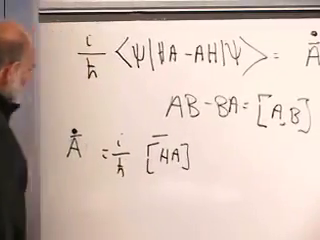
\includegraphics[width=0.74\textwidth]{lecture_09_figure_07.png}
\caption{期待値方程式と交換子\(AB-BA=[A,B]\)。}
\lectureframe{00:51:05}
\end{figure}

\begin{classroomqa}
\lecturetimestamp{00:49:13}
\audiencequestion{なぜこの方程式の交換子自体が期待値の中にあるのか？}
\lecturerresponse{交換子は演算子である。\(\bra{\psi}\)と\(\ket{\psi}\)の間に置かれた任意の演算子は期待値をもつので、\(\bra{\psi}[H,A]\ket{\psi}\)は単に現在の状態におけるその交換子の平均である。}
\end{classroomqa}

\subsection{保存則}

\(A=H\)と置く。演算子は常にそれ自身と交換する：
\begin{equation}
[H,H]=HH-HH=0.
\end{equation}
したがって
\begin{equation}
\boxed{
\frac{d}{dt}\langle H\rangle_t=0
}.
\end{equation}
ハミルトニアンの期待値は保存される。これが\(H\)をエネルギーと同定するために約束された構造的な理由である。すべての孤立系はハミルトニアンをもち、すべての時間非依存ハミルトニアンがこの保存則を与える。

より一般には、
\begin{equation}
[H,A]=0
\quad\Longrightarrow\quad
\frac{d}{dt}\langle A\rangle_t=0.
\end{equation}

\begin{classroomqa}
\lecturetimestamp{00:51:41}
\audiencequestion{\(H\)と交換するすべての演算子の集合の物理的解釈は何であり、それはエネルギー以外の量を含むか？}
\lecturerresponse{それらは系の保存観測量である。どれが現れるかはハミルトニアンに依存する。自由粒子は運動量を保存するが、力はその保存を破壊しうる。エネルギーは常に存在する。なぜなら\(H\)はそれ自身と交換するからである。追加の交換演算子は追加の対称性と保存則を表す。}
\end{classroomqa}

\section{磁場中の一つのスピン}

パウリ演算子
\begin{equation}
\boldsymbol{\sigma}
=(\sigma_1,\sigma_2,\sigma_3)
\end{equation}
をもつスピンを、固定された外部磁場\(\mathbf B\)の中に置く。磁気モーメントはスピンに比例する。ここで用いる規約では、
\begin{equation}
\boxed{
H=\frac{\mu}{2}\boldsymbol{\sigma}\cdot\mathbf B
}.
\end{equation}
因子\(1/2\)、符号、および電荷依存の尺度は\(\mu\)の定義に吸収してよい。磁場は古典的に扱う。大きな安定した磁石が\(\mathbf B\)を与え、その磁石の量子状態はモデル化しない。

\begin{figure}[htbp]
\centering
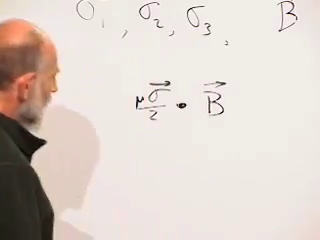
\includegraphics[width=0.68\textwidth]{lecture_09_figure_08.png}
\caption{磁気モーメント演算子は外部磁場と結合する。}
\lectureframe{01:01:45}
\end{figure}

磁場を第三軸に沿って選ぶ：
\begin{equation}
\mathbf B=B\hat{\mathbf z},
\qquad
H=\frac{\mu B}{2}\sigma_3.
\end{equation}
三つのスピン成分の期待値を追跡する。式を短くするため、
\begin{equation}
s_i(t)=\langle\sigma_i\rangle_t.
\end{equation}
と書く。縦成分は
\begin{equation}
\dot s_3
=
\frac{i}{\hbar}\langle[H,\sigma_3]\rangle
=0,
\end{equation}
に従う。なぜなら\(H\)は\(\sigma_3\)に比例するからである。磁場に沿ったスピンの射影は固定されている。幾何学的には、平均スピンの先端は磁場軸のまわりの固定された開き角の円錐上にとどまらなければならない。

\begin{figure}[htbp]
\centering
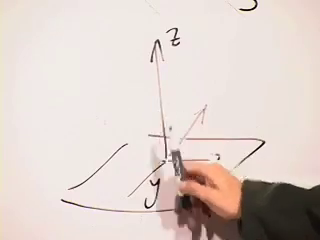
\includegraphics[width=0.58\textwidth]{lecture_09_figure_09.png}
\caption{固定された縦スピンは磁場軸のまわりの円錐上の運動を残す。}
\lectureframe{01:04:45}
\end{figure}

第一の横成分については、
\begin{equation}
\dot s_1
=
\frac{i\mu B}{2\hbar}
\langle[\sigma_3,\sigma_1]\rangle.
\end{equation}
交換子は
\begin{equation}
\begin{aligned}
\sigma_3&=
\begin{pmatrix}1&0\\0&-1\end{pmatrix},
&
\sigma_1&=
\begin{pmatrix}0&1\\1&0\end{pmatrix},\\[0.5em]
\sigma_2&=
\begin{pmatrix}0&-i\\i&0\end{pmatrix}.
\end{aligned}
\end{equation}
から直接確かめられる。実際、
\begin{equation}
\sigma_3\sigma_1=i\sigma_2,
\qquad
\sigma_1\sigma_3=-i\sigma_2,
\end{equation}
なので
\begin{equation}
[\sigma_3,\sigma_1]=2i\sigma_2.
\end{equation}
したがって、
\begin{equation}
\dot s_1=-\frac{\mu B}{\hbar}s_2.
\end{equation}
同様に、\([\sigma_3,\sigma_2]=-2i\sigma_1\)を用いて、
\begin{equation}
\dot s_2=\frac{\mu B}{\hbar}s_1.
\end{equation}

\begin{figure}[htbp]
\centering
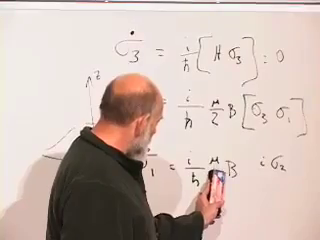
\includegraphics[width=0.72\textwidth]{lecture_09_figure_10.png}
\caption{横方向の運動方程式に至るパウリ交換子の計算。}
\lectureframe{01:09:35}
\end{figure}

\begin{equation}
\Omega=\frac{\mu B}{\hbar}.
\end{equation}
と置く。三つの方程式は
\begin{equation}
\dot s_1=-\Omega s_2,
\qquad
\dot s_2=\Omega s_1,
\qquad
\dot s_3=0.
\end{equation}
横振幅\(s_\perp\)をもつ解は
\begin{equation}
s_1(t)=s_\perp\cos(\Omega t+\varphi),
\qquad
s_2(t)=s_\perp\sin(\Omega t+\varphi),
\end{equation}
であり、\(s_3\)は定数である。

\begin{figure}[htbp]
\centering
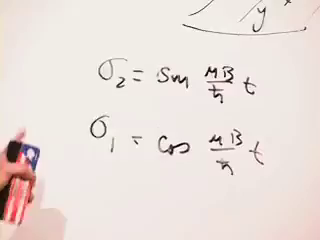
\includegraphics[width=0.64\textwidth]{lecture_09_figure_11.png}
\caption{横スピン成分は角振動数 \(\mu B/\hbar\) のサイン--コサイン対をなす。}
\lectureframe{01:11:45}
\end{figure}

したがって平均スピンは、ジャイロスコープのように磁場のまわりを歳差運動する。磁場を\(z\)に沿って選ぶことは、単なる便宜にすぎなかった。任意の方向の磁場に対して、\(\mathbf B\)に平行な成分は保存され、垂直な成分はそのまわりを回転する。

\begin{classroomqa}
\lecturetimestamp{01:13:02}
\audiencequestion{サインとコサインの解は、余分な位相を含むべきでしょうか。}
\lecturerresponse{はい。位相\(\varphi\)は横平面内の初期方向を指定し、あるいは同等に、\(t=0\)と呼ばれる時刻の選び方を指定する。それをゼロに設定することは、スピンがある特定の横軸に沿って始まるように選ぶことにすぎない。}
\end{classroomqa}

\subsection{準備と測定}

アンサンブルが\(\sigma_1\)の\(+1\)固有状態に準備されているとしよう。\(t=0\)において、\(\sigma_1\)の測定は確実に\(+1\)を返すが、\(\sigma_2\)または\(\sigma_3\)の測定は\(\pm1\)に対して等しい確率を与える。歳差運動の四分の一周期の後、状態は\(\sigma_2\)の\(+1\)固有状態へと回転している。そのとき\(\sigma_2\)は確実であり、\(\sigma_1\)は最大に不確定である。さらに四分の一周期の後、それは\(\sigma_1\)の\(-1\)固有状態に達する。したがって回転する期待値は、直接的な操作的意味をもつ。

\begin{classroomqa}
\lecturetimestamp{01:14:04}
\audiencequestion{期待値が多数の電子を必要とするなら、アンサンブルの各成員は異なる位相をもち、歳差運動を洗い流してしまわないでしょうか。}
\lecturerresponse{すべての成員に対して同じ実験が行われる場合には、そうはならない。同一の準備はすべての電子に同じ初期状態を与え、したがって同じ位相発展を与える。それらの初期位相が制御されていないなら、そのアンサンブルは純粋な準備ではなく、混合状態であり、位相緩和が横方向の平均を減少させうる。}
\end{classroomqa}

\section{二つの結合したスピン}

次に二つのスピンを考えよう。それらがもつれていると言うだけでは、それらが何をするかを予測するには十分でない。力学にはハミルトニアンが必要である。

\begin{classroomqa}
\lecturetimestamp{01:16:49}
\audiencequestion{二つの電子がもつれ合い、任意の共通軸に沿って反対の結果が生じるなら、それはそれらの運動が常に\(180^\circ\)位相がずれていることを意味するのでしょうか。}
\lecturerresponse{もつれだけからは、いかなる力学的結論も導かれない。述べられた反相関は一重項状態を記述するが、その後の発展はエネルギー演算子に依存する。まず外部磁場があるのか、スピン間の相互作用があるのか、あるいはその両方があるのかを指定しなければならない。}
\end{classroomqa}

各スピンが他方の感じる有効磁場を与える、単純な等方的相互作用を取ろう。
\begin{equation}
\boxed{
H=J\,\boldsymbol{\sigma}\cdot\boldsymbol{\tau}
=
J\left(
\sigma_1\tau_1+\sigma_2\tau_2+\sigma_3\tau_3
\right)
}.
\end{equation}
演算子\(\boldsymbol{\sigma}\)は第一のスピンに作用し、\(\boldsymbol{\tau}\)は第二のスピンに作用する。結合\(J\)はエネルギーの尺度を定める。その値と符号は指定しないままにしておく。

\begin{figure}[htbp]
\centering
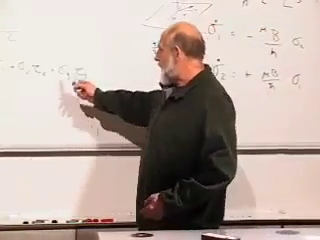
\includegraphics[width=0.75\textwidth]{lecture_09_figure_12.png}
\caption{等方的な二スピン相互作用\(H\propto\boldsymbol{\sigma}\cdot\boldsymbol{\tau}\)。}
\lectureframe{01:19:20}
\end{figure}

\begin{classroomqa}
\lecturetimestamp{01:17:49}
\audiencequestion{二つのもつれた電子を一様な磁場に置くと、必ずそれらはもつれが解けるのでしょうか。}
\lecturerresponse{必ずしもそうではない。磁場はハミルトニアンを変え、特にそれが強い場合にはスピンを整列させようとしうるが、一様な磁場におけるユニタリ発展それ自体はもつれの喪失を保証しない。答えは完全なハミルトニアンと初期状態に依存する。}
\end{classroomqa}

\subsection{三重項と一重項のエネルギー}

二スピンヒルベルト空間の次元は四である。相互作用は三重項--一重項基底において対角的である。
\begin{align}
\ket{T_+}&=\ket{\uparrow\uparrow}, \\
\ket{T_0}&=
\frac{\ket{\uparrow\downarrow}+\ket{\downarrow\uparrow}}{\sqrt2}, \\
\ket{T_-}&=\ket{\downarrow\downarrow}, \\
\ket{S}&=
\frac{\ket{\uparrow\downarrow}-\ket{\downarrow\uparrow}}{\sqrt2}.
\end{align}
三つの三重項状態は一つのエネルギー\(E_T\)を共有し、一重項は別のエネルギー\(E_S\)をもつ。したがって四つの独立な固有ベクトルがあるが、異なるエネルギー準位は二つだけである。三重項準位は三重に縮退している。

\begin{figure}[htbp]
\centering
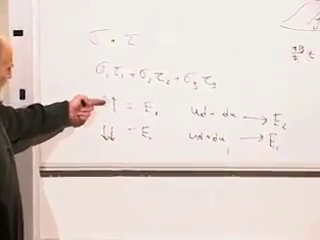
\includegraphics[width=0.74\textwidth]{lecture_09_figure_13.png}
\caption{結合したスピンのハミルトニアンは、縮退した三重項準位と別個の一重項準位をもつ。}
\lectureframe{01:20:30}
\end{figure}

\begin{classroomqa}
\lecturetimestamp{01:21:16}
\audiencequestion{初期状態がすでに一重項エネルギー固有状態である場合、何が起こるのでしょうか。}
\lecturerresponse{それは一重項のままであり、位相\(e^{-iE_St/\hbar}\)だけを獲得する。任意の単一エネルギー固有状態と同様に、ケット全体がその共通位相で掛けられるからといって、その可測な性質が変わるわけではない。}
\end{classroomqa}

\begin{classroomqa}
\lecturetimestamp{01:21:54}
\audiencequestion{この計算の間、外部磁場は二スピン系にエネルギーを供給するのでしょうか。}
\lecturerresponse{解いている例には外部磁場はない。議論されている唯一の場は、\(J\,\boldsymbol{\sigma}\cdot\boldsymbol{\tau}\)で表される相互相互作用である。外部磁場を加えることは、\(H\)に別の項を加え、異なる問題を定義することになる。}
\end{classroomqa}

\subsection{一つのスピンが上、一つが下から始める}

エネルギー固有状態は位相を得るだけであるから、エネルギー固有状態ではない積状態を選ぶ：
\begin{equation}
\ket{\psi(0)}=\ket{\uparrow\downarrow}.
\end{equation}
それを関連する2つの固有ベクトルに分解する：
\begin{equation}
\boxed{
\ket{\uparrow\downarrow}
=
\frac{1}{\sqrt2}\ket{T_0}
+
\frac{1}{\sqrt2}\ket{S}
}.
\end{equation}

\begin{figure}[htbp]
\centering
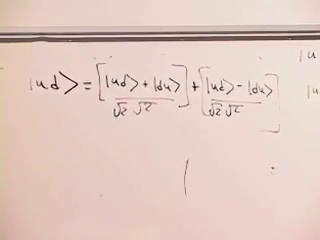
\includegraphics[width=0.76\textwidth]{lecture_09_figure_14.png}
\caption{積状態\(\ket{\uparrow\downarrow}\)を三重項成分と一重項成分に分解したもの。}
\lectureframe{01:24:30}
\end{figure}

各エネルギー成分は今やそれぞれ自身の位相を受け取る：
\begin{equation}
\ket{\psi(t)}
=
\frac{e^{-iE_Tt/\hbar}}{\sqrt2}\ket{T_0}
+
\frac{e^{-iE_St/\hbar}}{\sqrt2}\ket{S}.
\end{equation}

\begin{classroomqa}
\lecturetimestamp{01:25:59}
\audiencequestion{三重項エネルギー\(E_T\)と一重項エネルギー\(E_S\)のどちらが大きいか？}
\lecturerresponse{それは結合の符号に依存する。\(H=J\,\boldsymbol{\sigma}\cdot\boldsymbol{\tau}\)で\(J>0\)の場合、一重項が低く三重項が高く、符号を逆にすると順序も逆になる。両方のエネルギーに定数を加えても全体の位相が変わるだけなので、遷移確率を変えることなくどちらの準位もゼロに設定できる。}
\end{classroomqa}

積基底に戻る：
\begin{align}
\ket{\psi(t)}
&=
\frac12
\left(
e^{-iE_Tt/\hbar}+e^{-iE_St/\hbar}
\right)\ket{\uparrow\downarrow} \\
&\quad+
\frac12
\left(
e^{-iE_Tt/\hbar}-e^{-iE_St/\hbar}
\right)\ket{\downarrow\uparrow}.
\end{align}

\begin{figure}[htbp]
\centering
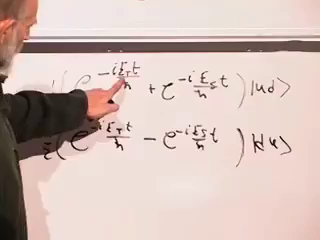
\includegraphics[width=0.76\textwidth]{lecture_09_figure_15.png}
\caption{時間発展した状態を\(\ket{\uparrow\downarrow}\)、\(\ket{\downarrow\uparrow}\)基底で再構成したもの。}
\lectureframe{01:30:40}
\end{figure}

\(t=0\)では、\(\ket{\downarrow\uparrow}\)の係数は消えるが、それは必然である。より後の時刻では、一重項成分と三重項成分の間の相対位相によりこの係数が成長する。平均エネルギーと分裂を定義すると、
\begin{equation}
\overline E=\frac{E_T+E_S}{2},
\qquad
\Delta E=E_T-E_S.
\end{equation}
平均エネルギーの位相をくくり出すと
\begin{equation}
\boxed{
\begin{aligned}
\ket{\psi(t)}
&=e^{-i\overline E t/\hbar}\Biggl[
\cos\!\left(\frac{\Delta E\,t}{2\hbar}\right)
\ket{\uparrow\downarrow}
\\
&\qquad
-i\sin\!\left(\frac{\Delta E\,t}{2\hbar}\right)
\ket{\downarrow\uparrow}
\Biggr]
\end{aligned}
}.
\end{equation}

\begin{figure}[H]
\centering
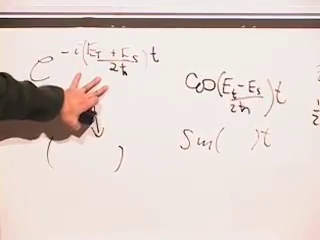
\includegraphics[width=0.76\textwidth]{lecture_09_figure_16.png}
\caption{平均エネルギーは共通の位相となり、一重項--三重項分裂はサインとコサインの振幅に現れる。}
\lectureframe{01:35:15}
\end{figure}

因子\(e^{-i\overline E t/\hbar}\)はケット全体に共通であり、すべての確率から落ちる。測定可能な確率は
\begin{equation}
P_{\uparrow\downarrow}(t)
=
\cos^2\!\left(\frac{\Delta E\,t}{2\hbar}\right),
\qquad
P_{\downarrow\uparrow}(t)
=
\sin^2\!\left(\frac{\Delta E\,t}{2\hbar}\right).
\end{equation}
状態は\(\ket{\uparrow\downarrow}\)から\(\ket{\downarrow\uparrow}\)へ、そしてまた戻るという振動を、エネルギー差のみで決まる速さで行う。中間の時刻では両方の振幅が非ゼロであり、特別な瞬間を除いて2つのスピンはもつれている。

この計算は一般的な方法を示している。物理的な問いが立てられている基底を選び、初期状態をハミルトニアンの固有ベクトルで展開し、各固有ベクトルにそれぞれの位相を与え、その後で各部分を測定基底で再結合する。ハミルトニアンが対角化されれば、量子力学の時間発展は系統的になる。観測可能な運動はすべて相対位相によって担われる。
